\documentclass{beamer}
\usetheme{Madrid}
\usepackage{lmodern}
\usepackage{hyperref}
\usepackage{apacite}
\usepackage[utf8]{inputenc}
\usepackage[spanish]{babel}

\usepackage{xcolor}
\setbeamertemplate{background}{\tikz[overlay,remember picture]\node[opacity=0.2]at (current page.center){
\includegraphics[width=13cm]{KL.png}};}
\usepackage{tikz}
\usepackage{kantlipsum}

\setbeamercolor{normal text}{fg=black}

\begin{document}
\colorlet{beamer@blendedblue}{blue!46!green}
\setbeamercolor{normal text}{fg=black}

\setbeamercolor{frametitle}{fg=white, bg=blue!46!green}
\setbeamercolor*{title}{bg=blue!46!green, fg=white}

\setbeamercolor{section in toc}{fg=black}

\author[Juan C. Correa \textcolor{white}{(\url{https://correajc.com}})]{Juan C. Correa, Ph.D.}
\title[TREME]{TREME}
\subtitle{Tecnologías Reproducibles para la Enseñanza \\de la Metodología y la Estadística}
	%\subtitle{}
\institute[]{Fundación Universitaria Konrad Lorenz\\
	\color{blue}\Email  \href{mailto:juanc.correan@konradlorenz.edu.co}{juanc.correan@konradlorenz.edu.co}}
\pgfdeclareimage[height=0.5cm]{KL}{KL}
\logo{\pgfuseimage{KL}}
\setbeamertemplate{caption}[numbered]
\date[Bogotá, Mayo-2021]{}

%\subject{}
\setbeamercolor{background canvas}{bg=white}
%\setbeamertemplate{navigation symbols}{}

\begin{frame}
	\titlepage
\end{frame}

\begin{frame}
\begin{block}{Objetivo del Curso}
\vspace{0.3cm}
Comprender las nuevas habilidades y competencias prácticas que facilitan y enriquecen la enseñanza y aprendizaje de contenidos metodológicos y estadísticos desde una óptica reproducible.  
\end{block}
\end{frame}

\begin{frame}
\frametitle{Agenda} 
\tableofcontents
\end{frame}


% \begin{frame}
% \Huge
% \centering
% \textcolor{blue!46!green}{Elementos de Alfabetización Estadística en Psicología}
% \end{frame}

\section{Motivación}
\begin{frame}{Motivación}
\citeauthor{Baker2016} \citeyear{Baker2016} mostró que muchos ``hallazgos científicos publicados'' realmente no son reproducibles.
\vspace{0.5cm}
\begin{figure}
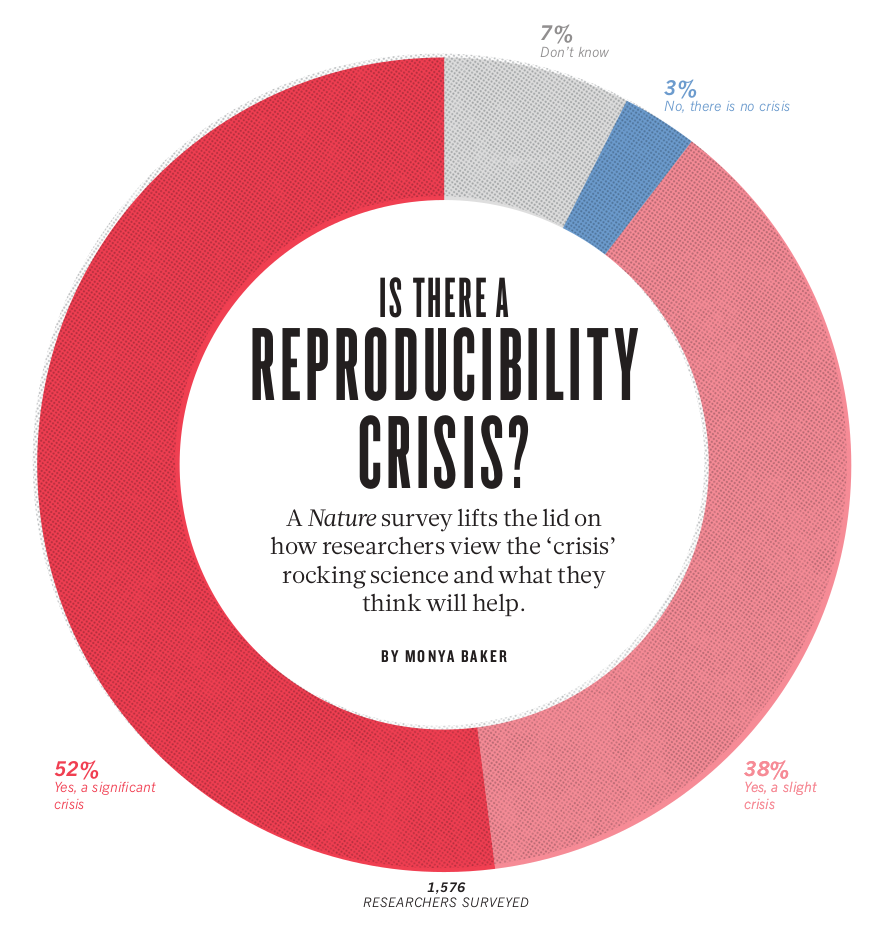
\includegraphics[width=.4\textwidth]{rc.png}
\end{figure}
\tiny
\textcolor{blue}{\url{https://www.nature.com/news/1-500-scientists-lift-the-lid-on-reproducibility-1.19970}}
\end{frame}

\begin{frame}{Motivación}
Cuando se repitieron (replicar) los análisis de 100 estudios experimentales y correlaciones publicados en tres revistas de gran prestigio en psicología, se encontraron que los resultados no coincidían \cite{Open2015}.
\vspace{0.5cm}
\begin{figure}

\includegraphics[width=.7\textwidth]{OSC.png}
\end{figure}
\end{frame}

\begin{frame}{Motivación}
``Las afirmaciones científicas no deben ganar credibilidad por el estatus o la autoridad de su creador, sino por la replicabilidad de sus pruebas de apoyo. Incluso la investigación de calidad ejemplar puede tener hallazgos empíricos irreproducibles debido a errores aleatorios o sistemáticos.''
\end{frame}

\begin{frame}{Motivación}
\begin{figure}
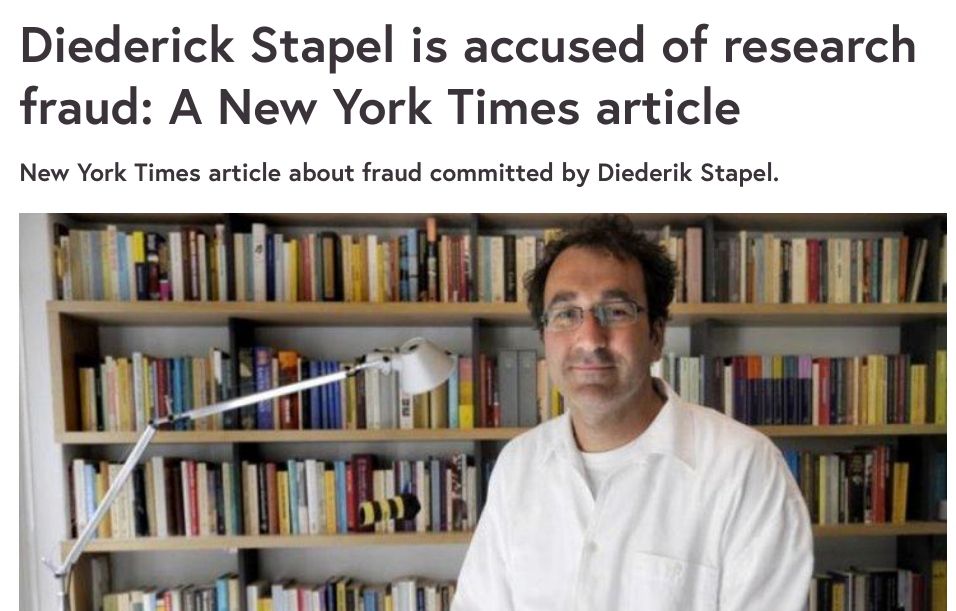
\includegraphics[width=.7\textwidth]{stapel.png}
\end{figure}
\scriptsize
\textcolor{blue}{\url{https://www.apa.org/science/about/psa/2011/12/diederik-stapel}}
\end{frame}

\begin{frame}{Motivación}
Casos como el de Diedrick Stapel, junto a la crisis de reproducibilidad, han motivado a gran parte de la comunidad académica a aumentar los estándares científicos de la disciplina, a través del empleo de tecnologías que permiten la replicabilidad y reproducibilidad de los hallazgos \cite{Epskamp2019}.
\end{frame}

\begin{frame}{Implicaciones}
Por \textcolor{blue!46!green}{\textbf{Reproducibilidad}} debe entenderse la posibilidad de reproducir los resultados numéricos originalmente publicados usando los mismos datos y aplicando los mismos códigos o procedimientos empleados por el investigador.   \\
\vspace{0.5cm}
Por \textcolor{blue!46!green}{\textbf{Replicabilidad}} debe entenderse la posibilidad de llegar a las mismas conclusiones publicadas por el investigador cuando se reanalizan los mismos datos o se analizan datos nuevos.
\end{frame}

\section{Implicaciones para la Formación de Nuevas Generaciones}
\begin{frame}{Implicaciones}
Los conceptos de reproducibilidad y replicabilidad nos han llevado a entender que entre todas las formas de conocimiento que posee la humanidad (e.g., conocimiento empírico, conocimiento religioso, conocimiento jurídico), el método científico es la mejor forma que se tiene para corregir nuestros errores a la hora de estudiar el comportamiento humano. 
\end{frame}

\section{¿Qué se puede mejorar en la enseñanza?}
\begin{frame}{¿Qué se puede mejorar en la enseñanza?}
\begin{itemize}
\item Reemplazar el uso de software de licencia privativa (e.g., SPSS) por software de licencia abierta (e.g., Jasp, Jamovi, Gephi, R, Python). Con ello, las universidades, los docentes y los estudiantes se ahorran dinero. 
\end{itemize}
\begin{figure}
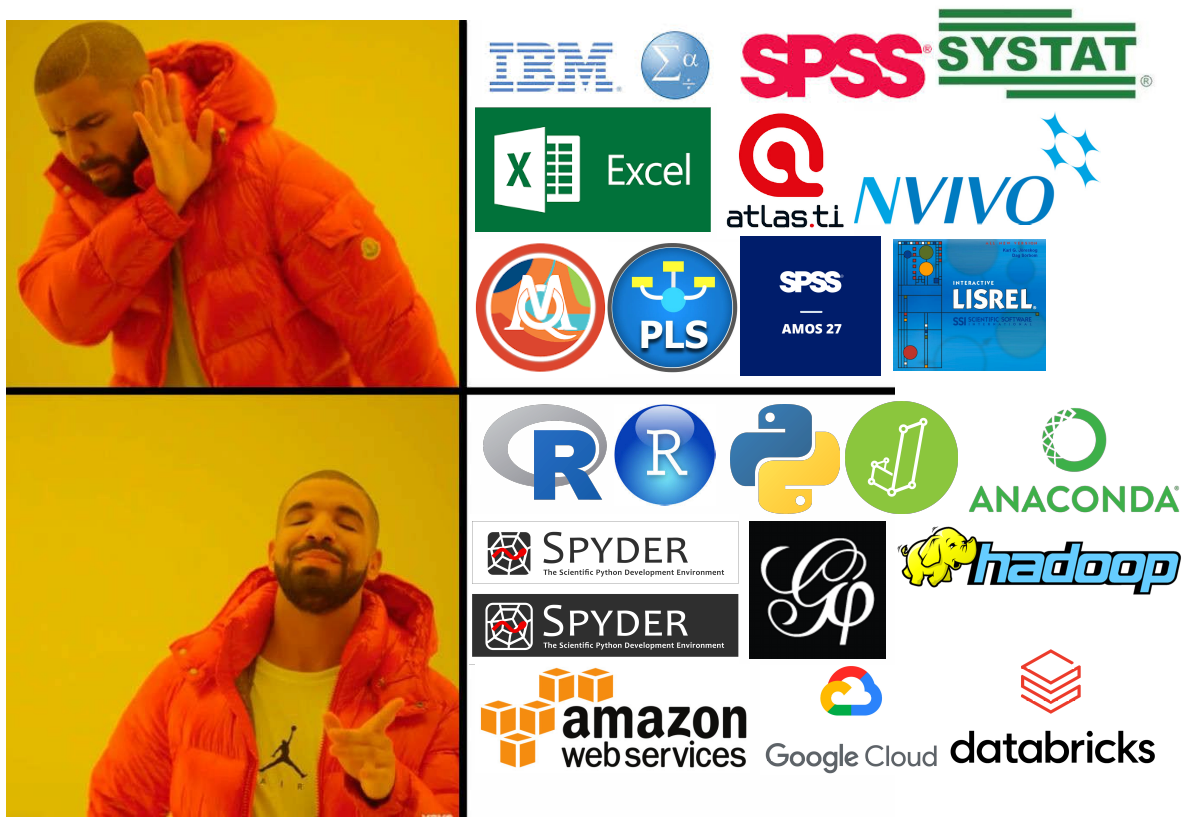
\includegraphics[width=.5\textwidth]{thisnot.png}
\end{figure}
\end{frame}

\begin{frame}{¿Qué se puede mejorar en la enseñanza?}
\begin{itemize}
\item Enseñar otros métodos contemporáneos para reportar propiedades psicométricas de tests psicológicos, cuestionarios, o encuestas \cite{Zhang2016}
\end{itemize}    
\begin{figure}

\includegraphics[width=.9\textwidth]{zhang.png}
\end{figure}
\end{frame}


\begin{frame}{¿Qué se puede mejorar en la enseñanza?}
\begin{itemize}
\item Enseñar otros métodos contemporáneos para el contraste de hipótesis que no dependan del modelo lineal general \cite{Mair2020}
\end{itemize}    
\begin{figure}
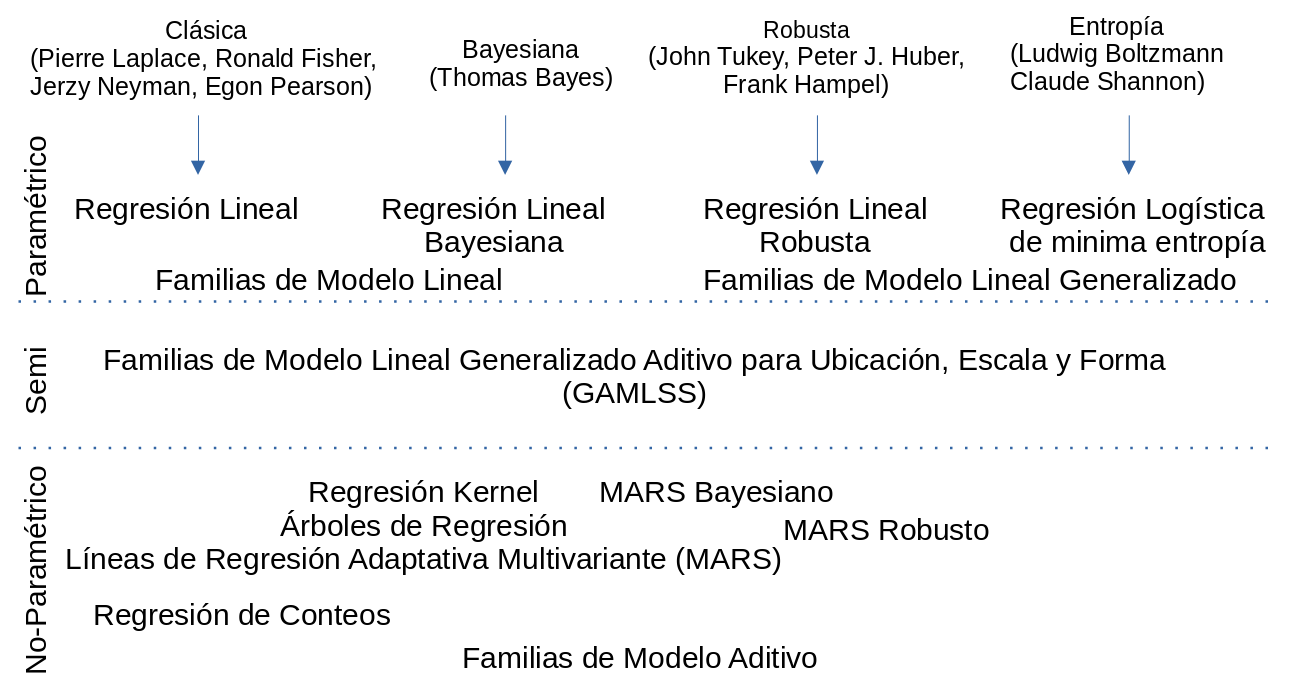
\includegraphics[width=.9\textwidth]{Arbol.png}
\end{figure}
\end{frame}


\begin{frame}{¿Qué se puede mejorar en la enseñanza?}
\begin{itemize}
\item Enseñar por qué la paradoja de Simpson y el cuarteto de Anscombe nos debe hacer reflexionar acerca de cómo debemos reportar resultados estadísticos \cite{Fulton2008}
\end{itemize}    
\begin{figure}
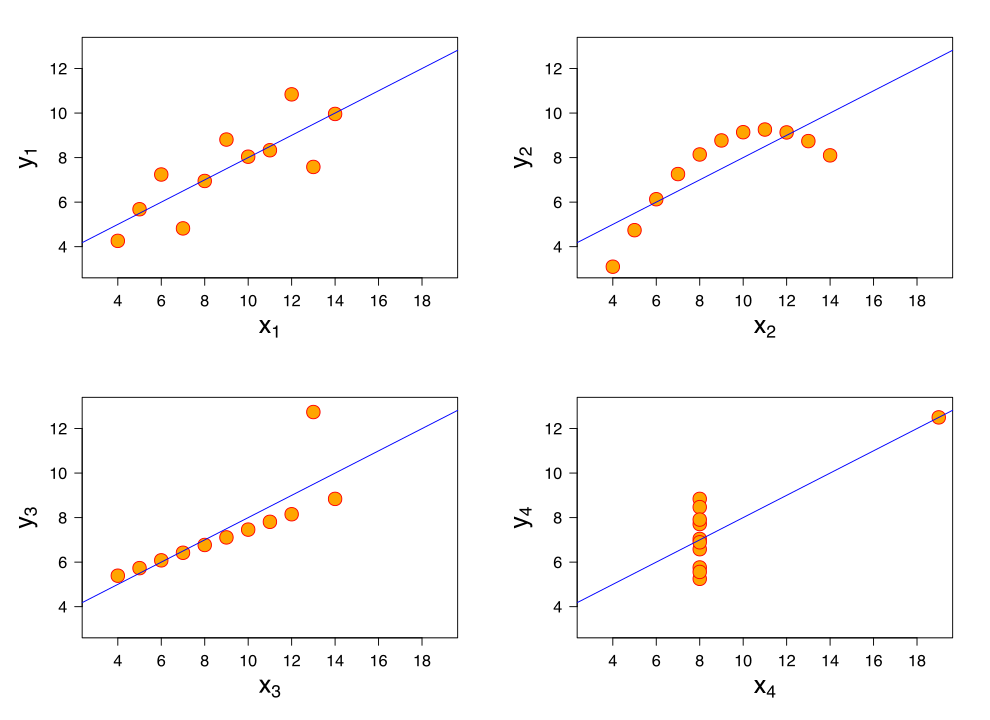
\includegraphics[width=.6\textwidth]{AQ.png}
\end{figure}
\end{frame}

\section{Las Nuevas Habilidades}
\begin{frame}{Las Nuevas Habilidades}
\begin{itemize}
\item Enseñar usando datos reales provenientes de fuentes acreditadas
\end{itemize}    
\begin{figure}

\includegraphics[width=.5\textwidth]{OWD.jpg}
\end{figure}
Se enseña a buscar datos como algo distinto de buscar información.
\end{frame}

\begin{frame}{Las Nuevas Habilidades}
\begin{itemize}
\item Enseñar a reproducir y replicar resultados publicados \cite{nosek2021}
\end{itemize}    
\begin{figure}
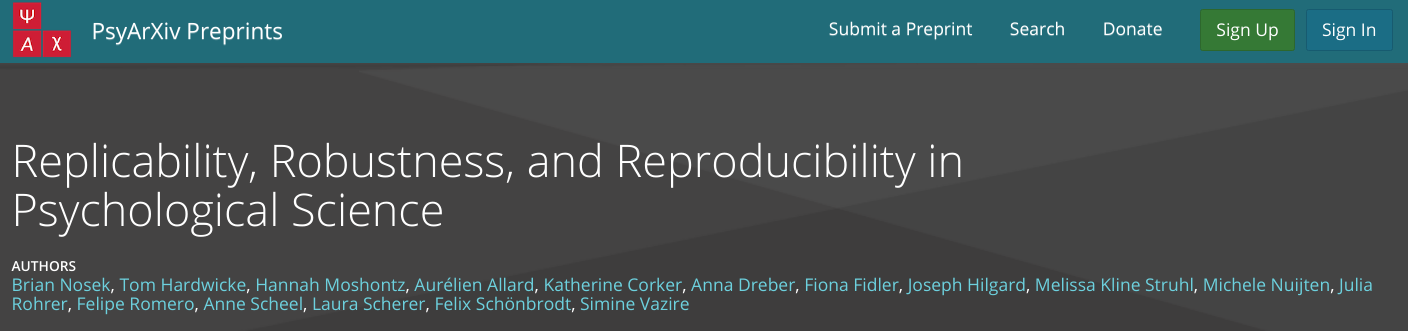
\includegraphics[width=1\textwidth]{rep.png}
\end{figure}
Se enseña el valor de los datos secundarios en comparación con el costo de obtener datos primarios.
\end{frame}


\begin{frame}{Las Nuevas Habilidades}
\begin{itemize}
\item Enseñar a analizar otros tipos de datos (e.g., textos, videos, fotos) \cite{Teichert2020}
\end{itemize}    
\begin{figure}
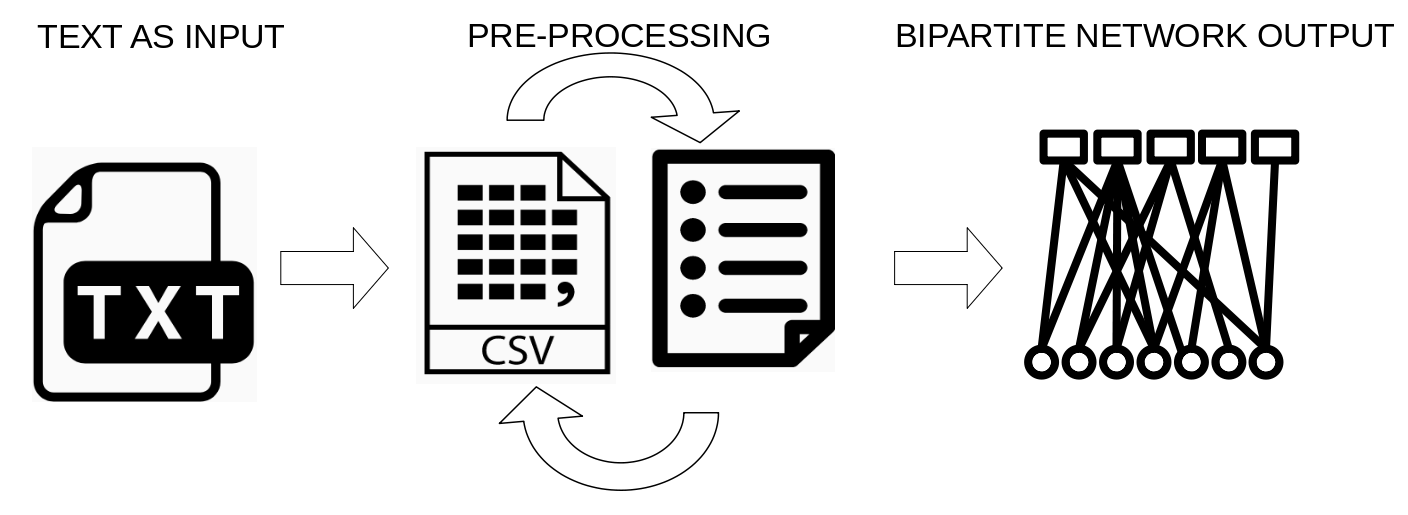
\includegraphics[width=.8\textwidth]{map.png}
\end{figure}
Se enseña una concepción de datos más amplia y versátil.
\end{frame}




\begin{frame}[allowframebreaks]{Referencias}
\tiny
\bibliographystyle{apacite}
\bibliography{refs} 
\end{frame}


\end{document}